\documentclass[aspectratio=169, handout]{beamer}

% PACKAGES -----------------------------------------------------------------------------------------

\usepackage{array}
\usepackage{caption}
\usepackage{ragged2e}
\usepackage{tikz}

% THEMING ------------------------------------------------------------------------------------------

% Beamer slide structure
\usetheme{Madrid}
\setbeamertemplate{navigation symbols}{}
\setbeamertemplate{caption}[numbered]
\setbeamertemplate{caption label separator}[period]

% Beamer colors
\usecolortheme{beaver}
\setbeamercolor{item}{fg=darkred}
\setbeamercolor{section in head/foot}{bg = white}

\setbeamercolor{frametitle}{fg=darkred,bg=}

% Beamer footer
\setbeamercolor{footer}{bg = white, fg = black}
\setbeamertemplate{footline}{
    \hbox{%
        \begin{beamercolorbox}[wd=.333333\paperwidth,ht=2.25ex,dp=1ex,left]{footer}
            \hspace{2ex}\insertshortauthor
        \end{beamercolorbox}%
        \begin{beamercolorbox}[wd=.333333\paperwidth,ht=2.25ex,dp=1ex,center]{footer}
            \insertshorttitle
        \end{beamercolorbox}%
        \begin{beamercolorbox}[wd=.333333\paperwidth,ht=2.25ex,dp=1ex,right]{footer}
            \insertframenumber\hspace{2ex}
        \end{beamercolorbox}
    }
}

% Other
\def\arraystretch{1.5}
\DeclareCaptionFont{darkred}{\color{darkred}}
\captionsetup{font=scriptsize,labelfont={darkred,scriptsize}}

% DOCUMENT INFORMATION -----------------------------------------------------------------------------

\title
    [Large Scale Hybrid Computing 25/26]
    {\large Cosmological Hydrodynamics at Exascale: A Trillion-Particle Leap in Capability}
\subtitle{\color{black} \small Large Scale Hybrid Computing 25/26}

\author[Humberto Gomes, José Lopes]{
    \begin{tabular}{lc}
        Humberto Gomes & \color{gray} pg59806 \\
        José Lopes     & \color{gray} pg59807 \\
    \end{tabular}
}

\institute{
    Department of Informatics -- School of Engineering -- University of Minho \\
    \vspace{0.5\baselineskip}
    
\includegraphics[height=1cm]{res/SchoolOfEngineering.pdf}
}
\date{\scriptsize April 9\textsuperscript{th} 2026}

\newif\ifplacelogo
\logo{
    \ifplacelogo
        \begin{tikzpicture}[overlay,remember picture]
        \node[anchor=north east, inner sep=0] at (current page.north east) {
            
\includegraphics[height=1cm]{res/SchoolOfEngineering.pdf}
        };
        \end{tikzpicture}
    \fi
}

% DOCUMENT CONTENTS --------------------------------------------------------------------------------

\begin{document}

\placelogofalse
\frame[plain]{\titlepage}
\placelogotrue

\begin{frame}{Table of contents}
    \tableofcontents
\end{frame}

\justifying

\section{Cosmological Simulations}

\begin{frame}{Cosmological Simulations}
    \begin{itemize}
        \item Simulating the formation and evolution of the structure of the Universe is crucial for
              interpreting results of cosmological surveys.
    \end{itemize}

    \vspace{1.5\baselineskip}
    \begin{minipage}{0.45\textwidth}
        \begin{center}
            \textbf{N-body Simulations}
        \end{center}
        \begin{itemize}
            \item Simulate only gravity;
            \item Low fidelity for current surveys.
        \end{itemize}
    \end{minipage}
    \begin{minipage}{0.5\textwidth}
        \begin{center}
            \textbf{Cosmological Hydrodynamic Simulations}
        \end{center}
        \begin{itemize}
            \item Simulates gas dynamics, star formation, ...
            \item 10--20$\times$ more computationally intensive.
        \end{itemize}
    \end{minipage}
\end{frame}

\section{Frontier-E Simulation}

\begin{frame}{Frontier-E -- Goals}
    \centering
    \vspace{\baselineskip}
    \begin{itemize}
        \item Frontier-E enables large-scale cosmological hydrodynamics through efficient exascale
              machine usage though CRK-HACC.
    \end{itemize}

    \begin{figure}
        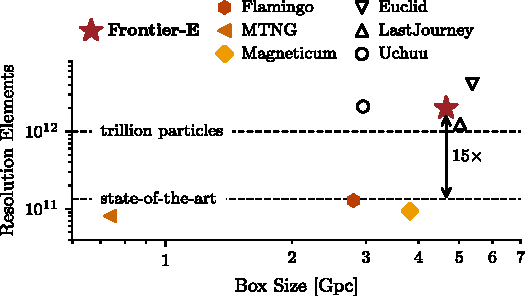
\includegraphics[width=0.6\textwidth]{res/Resolution.pdf}
        \caption{
            Box sizes and resolution elements of n-body (black) and hydrodynamic ({\color{darkred}
            colored}) simulations
        }
    \end{figure}
\end{frame}

\begin{frame}{Frontier-E -- Separation of Scale}
    \vspace{0.5\baselineskip}
    \begin{figure}
        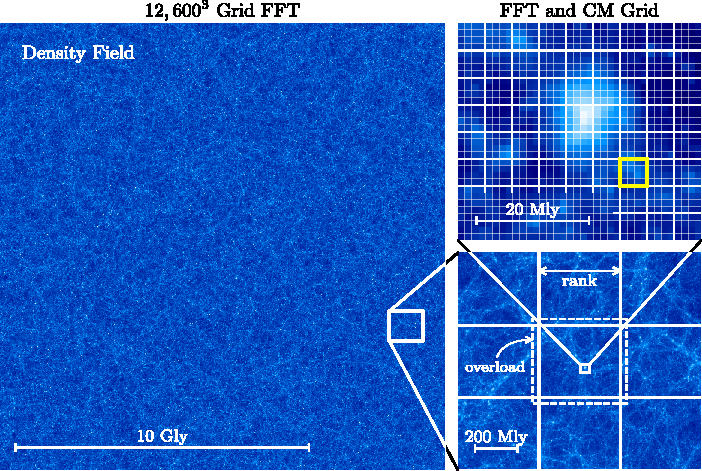
\includegraphics[width=0.65\textwidth]{res/SeparationOfScale.pdf}
        \caption{Domain subdivision and different interaction scales in Frontier-E}
    \end{figure}
\end{frame}

\begin{frame}{Frontier-E -- Innovations (I)}
    \vspace{\baselineskip}
    \begin{minipage}{0.6\textwidth}
        \centering
        \textbf{GPU Tree Solver}
        \begin{figure}
            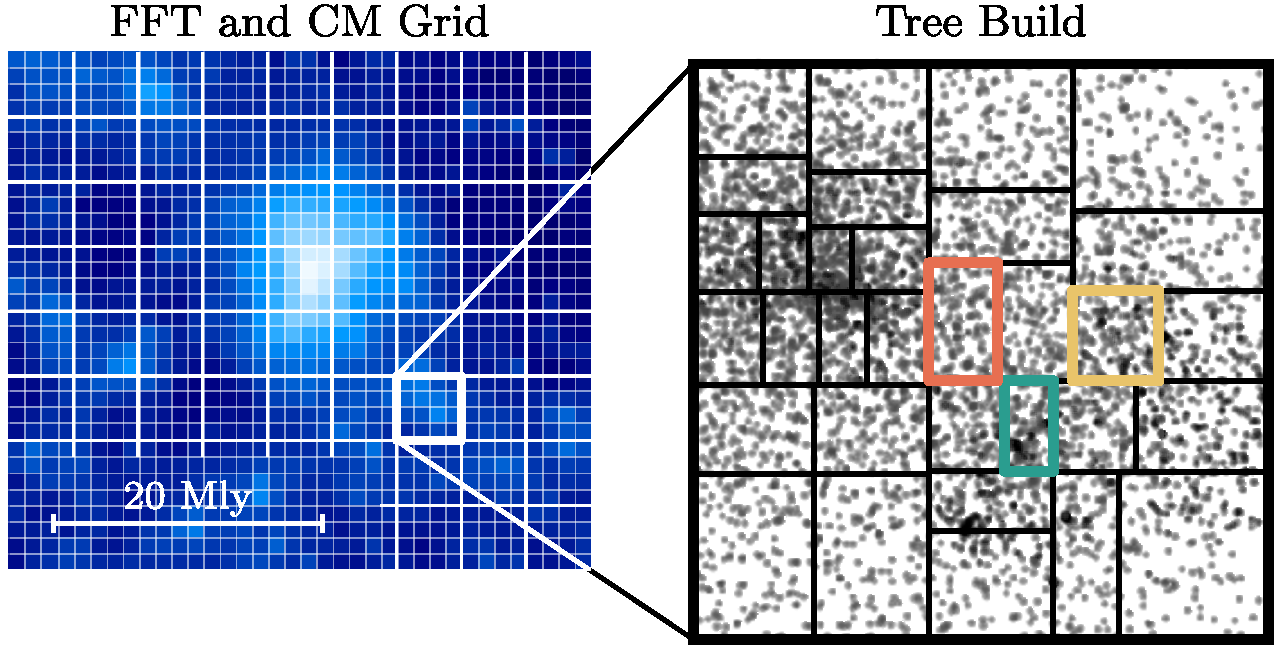
\includegraphics[width=0.9\textwidth]{res/GPUTreeSolver.pdf}
            \caption{GPU Tree leaves generated for one CM bin.}
        \end{figure}
    \end{minipage}
    \begin{minipage}{0.4\textwidth}
        \centering
        \textbf{Warp Splitting}
        \begin{figure}
            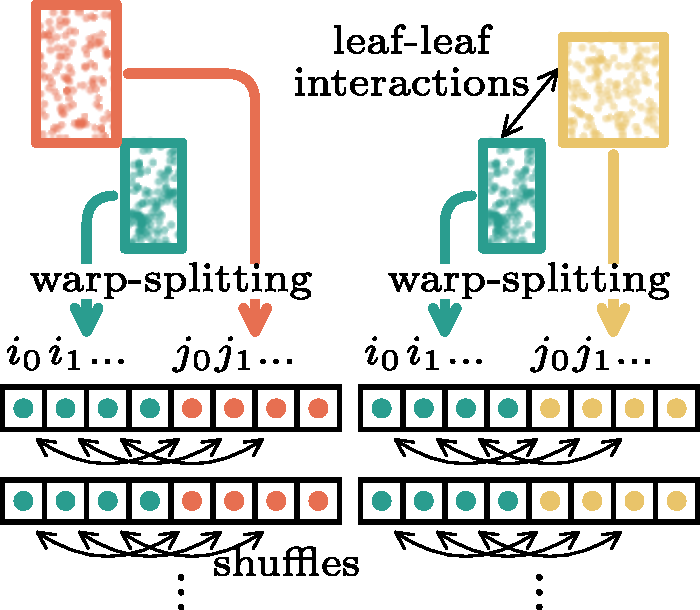
\includegraphics[width=0.8\textwidth]{res/WarpSplitting.pdf}
            \caption{Short-range GPU solver.}
        \end{figure}
    \end{minipage}
\end{frame}

\begin{frame}{Frontier-E -- Innovations (II)}
    \vspace{\baselineskip}
    \begin{minipage}{0.6\textwidth}
        \centering
        \textbf{In situ GPU-Accelerated End-to-End Analysis}
        \begin{figure}
            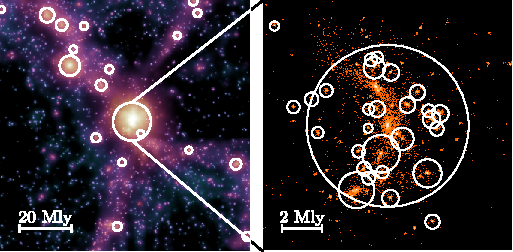
\includegraphics[width=0.9\textwidth]{res/GPUAnalysis.pdf}
            \caption{Halo (left) and galaxy (right) and detection}
        \end{figure}
    \end{minipage}
    \begin{minipage}{0.4\textwidth}
        \centering
        \textbf{Multi-Tiered I/O}

        \begin{figure}
            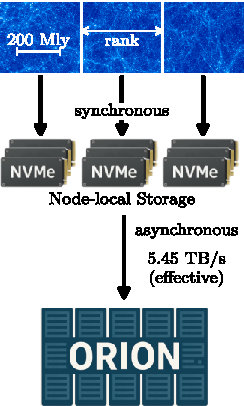
\includegraphics[width=0.55\textwidth]{res/TieredIO.pdf}
            \caption{Frontier-E storage tiers}
        \end{figure}
    \end{minipage}
\end{frame}

\section{Frontier Supercomputer}

\begin{frame}{Frontier Supercomputer}
    \vspace{\baselineskip}
    \begin{minipage}{0.45\textwidth}
        \centering
        \begin{figure}
            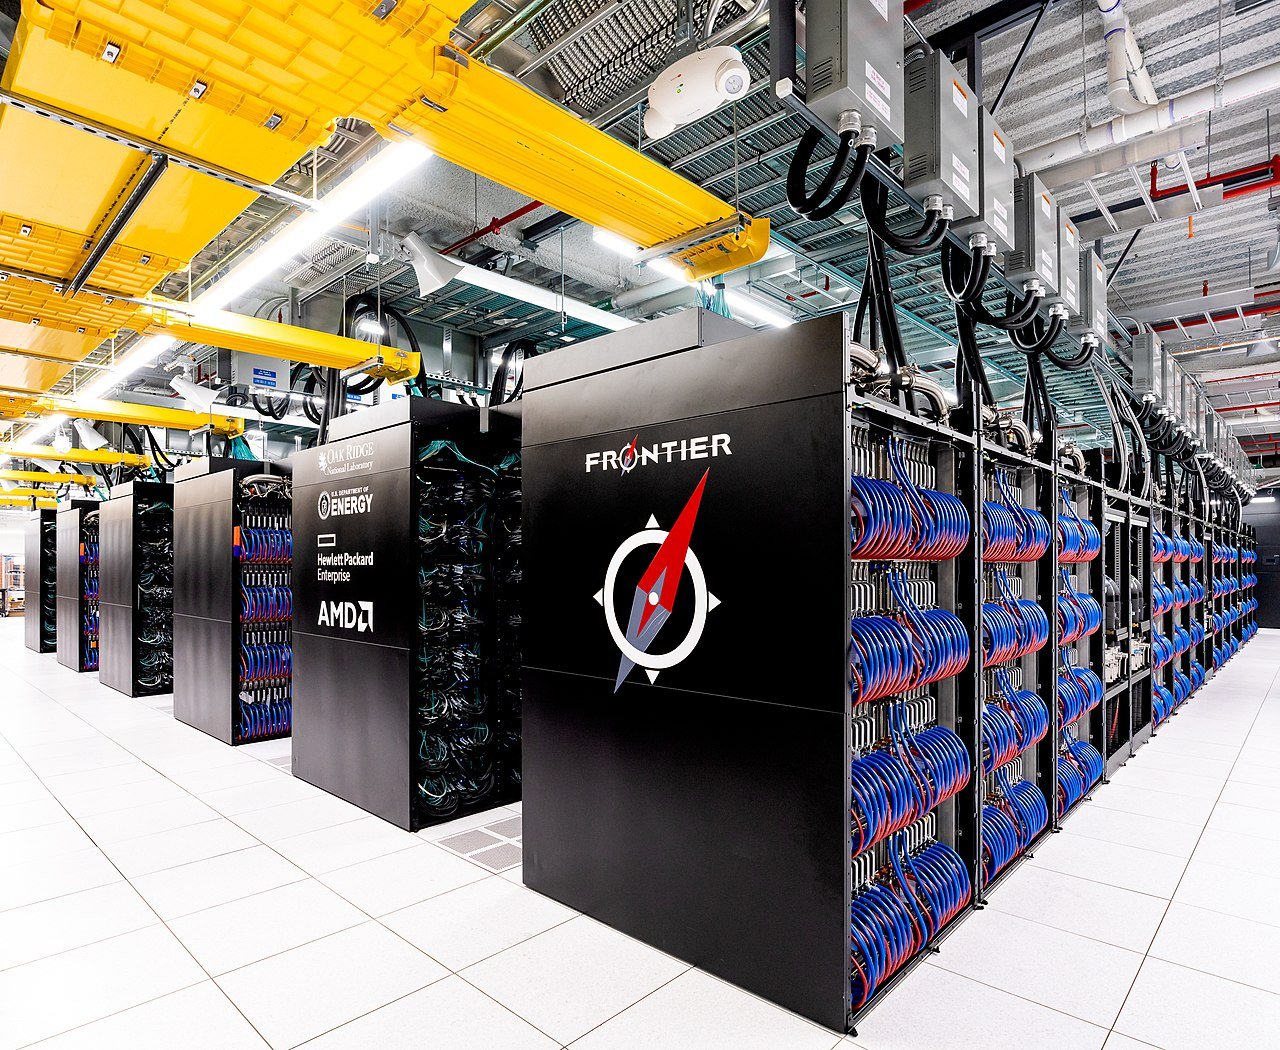
\includegraphics[width=0.95\textwidth]{res/Frontier.jpg}
            \caption{Frontier (Oak Ridge National Laboratory)}
        \end{figure}
    \end{minipage}
    \hfill
    \begin{minipage}{0.52\textwidth}
        \begin{tabular}{|cl|}
            \hline
            \multicolumn{2}{|c|}{128 -- 9000 nodes}        \\
            
\includegraphics[width=3ex]{res/icons/cpu.png} &
            64-core AMD EPYC Zen 3 ``Trento''              \\
            
\includegraphics[width=4ex]{res/icons/gpu.png} &
            4$\times$ AMD Instinct MI250X                  \\
            
\includegraphics[width=4ex]{res/icons/ram.png} &
            512 GiB DDR4 + 4$\times$ 64 GiB HBM2e          \\
            
\includegraphics[width=3ex]{res/icons/ssd.png} &
            2$\times$ NVMe SSD (4 GB/s writes)             \\
            \hline
            \multicolumn{1}{c}{
\includegraphics[width=3ex]{res/icons/lustre.png}} &
            \multicolumn{1}{l}{LustreFS PFS (4.6 TB/s writes)}                    \\
        \end{tabular}
    \end{minipage}
\end{frame}

\section{Results}

\begin{frame}{Results -- Parallel Scaling and Performance}
    \vspace{\baselineskip}
    \begin{minipage}{0.6\textwidth}
        \begin{figure}
            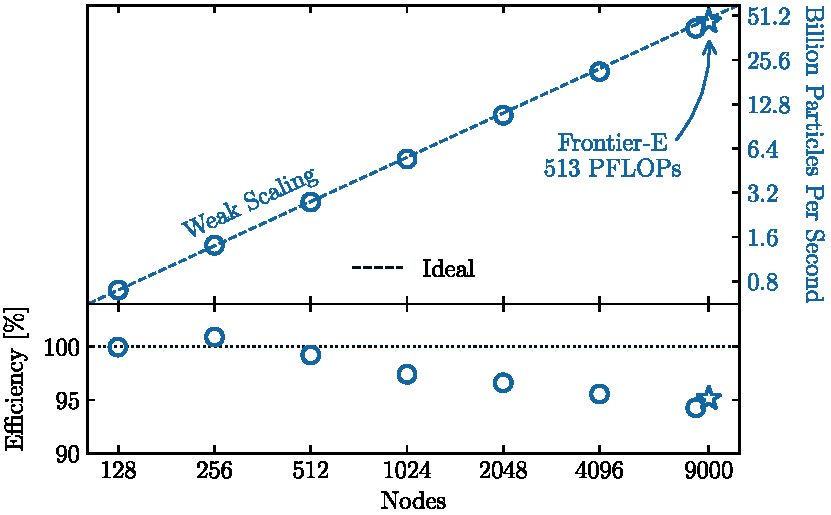
\includegraphics[width=\textwidth]{res/Scaling.pdf}
            \caption{Weak scalability on Frontier}
        \end{figure}
    \end{minipage}
    \begin{minipage}{0.38\textwidth}
        \hfill
        \small
        \begin{table}
            \begin{tabular}{|l|r|r|}
                \cline{2-3}
                \multicolumn{1}{c|}{} & PFLOPS &    \% \\ \hline
                Sustained             &  420.5 &  24.4 \\
                Peak                  &  513.1 &  29.8 \\
                Hardware Peak         & 1720.0 & 100.0 \\ \hline
            \end{tabular}
            \caption{Frontier supercomputer utilization}
        \end{table}
    \end{minipage}
\end{frame}

\begin{frame}{Results -- Time to Solution}
    \vspace{\baselineskip}
    \begin{minipage}{0.55\textwidth}
        \begin{figure}
            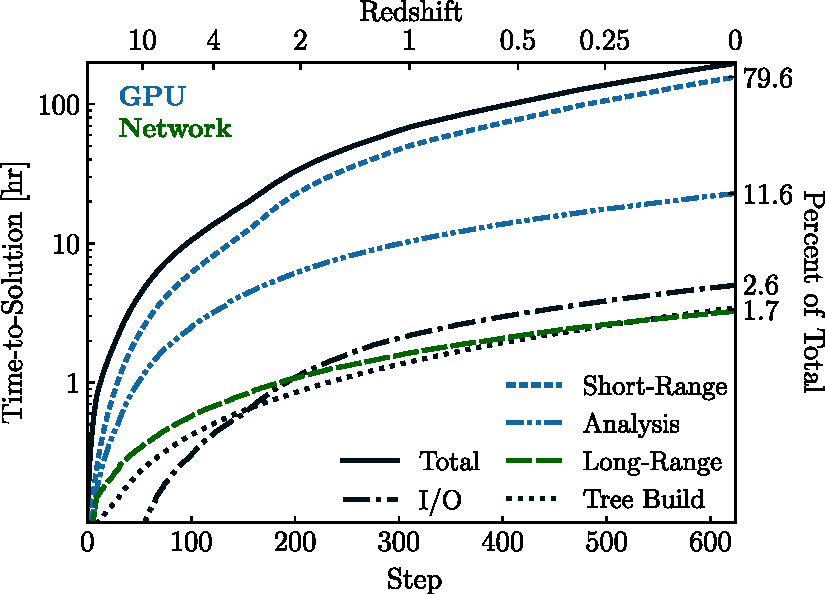
\includegraphics[width=\textwidth]{res/TimeToSolution.pdf}
            \caption{Cumulative time-to-solution of Frontier-E and its individual solvers}
        \end{figure}
    \end{minipage}
    \begin{minipage}{0.45\textwidth}
        \begin{itemize}
            \item 196 hours (8 days) of runtime;
            \item $> 90 \%$ of time in GPU operations;
        \end{itemize}
    \end{minipage}
\end{frame}

\begin{frame}{Results -- Resource Usage}
    \vspace{\baselineskip}
    \begin{minipage}[c]{0.5\textwidth}
        \centering
        \textbf{\hspace{4ex} I/O Usage}
        \begin{figure}
            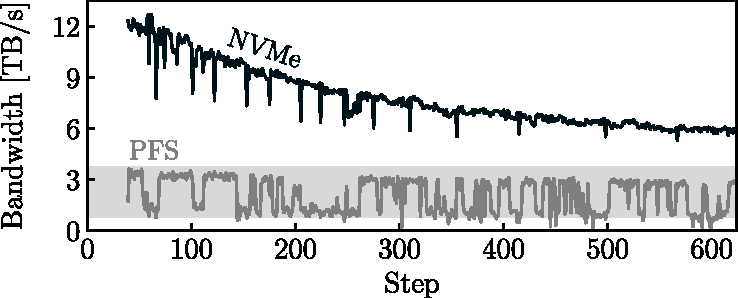
\includegraphics[width=\textwidth]{res/IOUsage.pdf}
            \caption{NVMe and PFS write bandwidth over time}
        \end{figure}
    \end{minipage}
    \begin{minipage}[c]{0.5\textwidth}
        \centering
        \textbf{GPU Usage}
        % \begin{figure}
        %     \includegraphics[width=0.35\textwidth]{res/Portability.pdf}
        %     \caption{GPU utilization across different GPU vendors}
        % \end{figure}
        \begin{figure}
            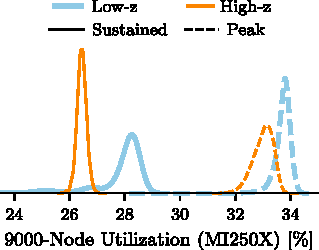
\includegraphics[width=0.8\textwidth]{res/GPUUtilization.pdf}
            \caption{GPU utilization at different simulation stages}
        \end{figure}
    \end{minipage}
\end{frame}

\section{Conclusion}

\begin{frame}{Conclusion}
    \vspace{\baselineskip}
    \begin{itemize}
        \item Frontier-E provides the resolution and realism needed for next-generation surveys;
        \item Peak and sustained FLOP ratios of 513 and 420 PFLOPS were achieved;
        \item Techniques developed applicable to other simulations.
    \end{itemize}
    \centering
    \begin{figure}
        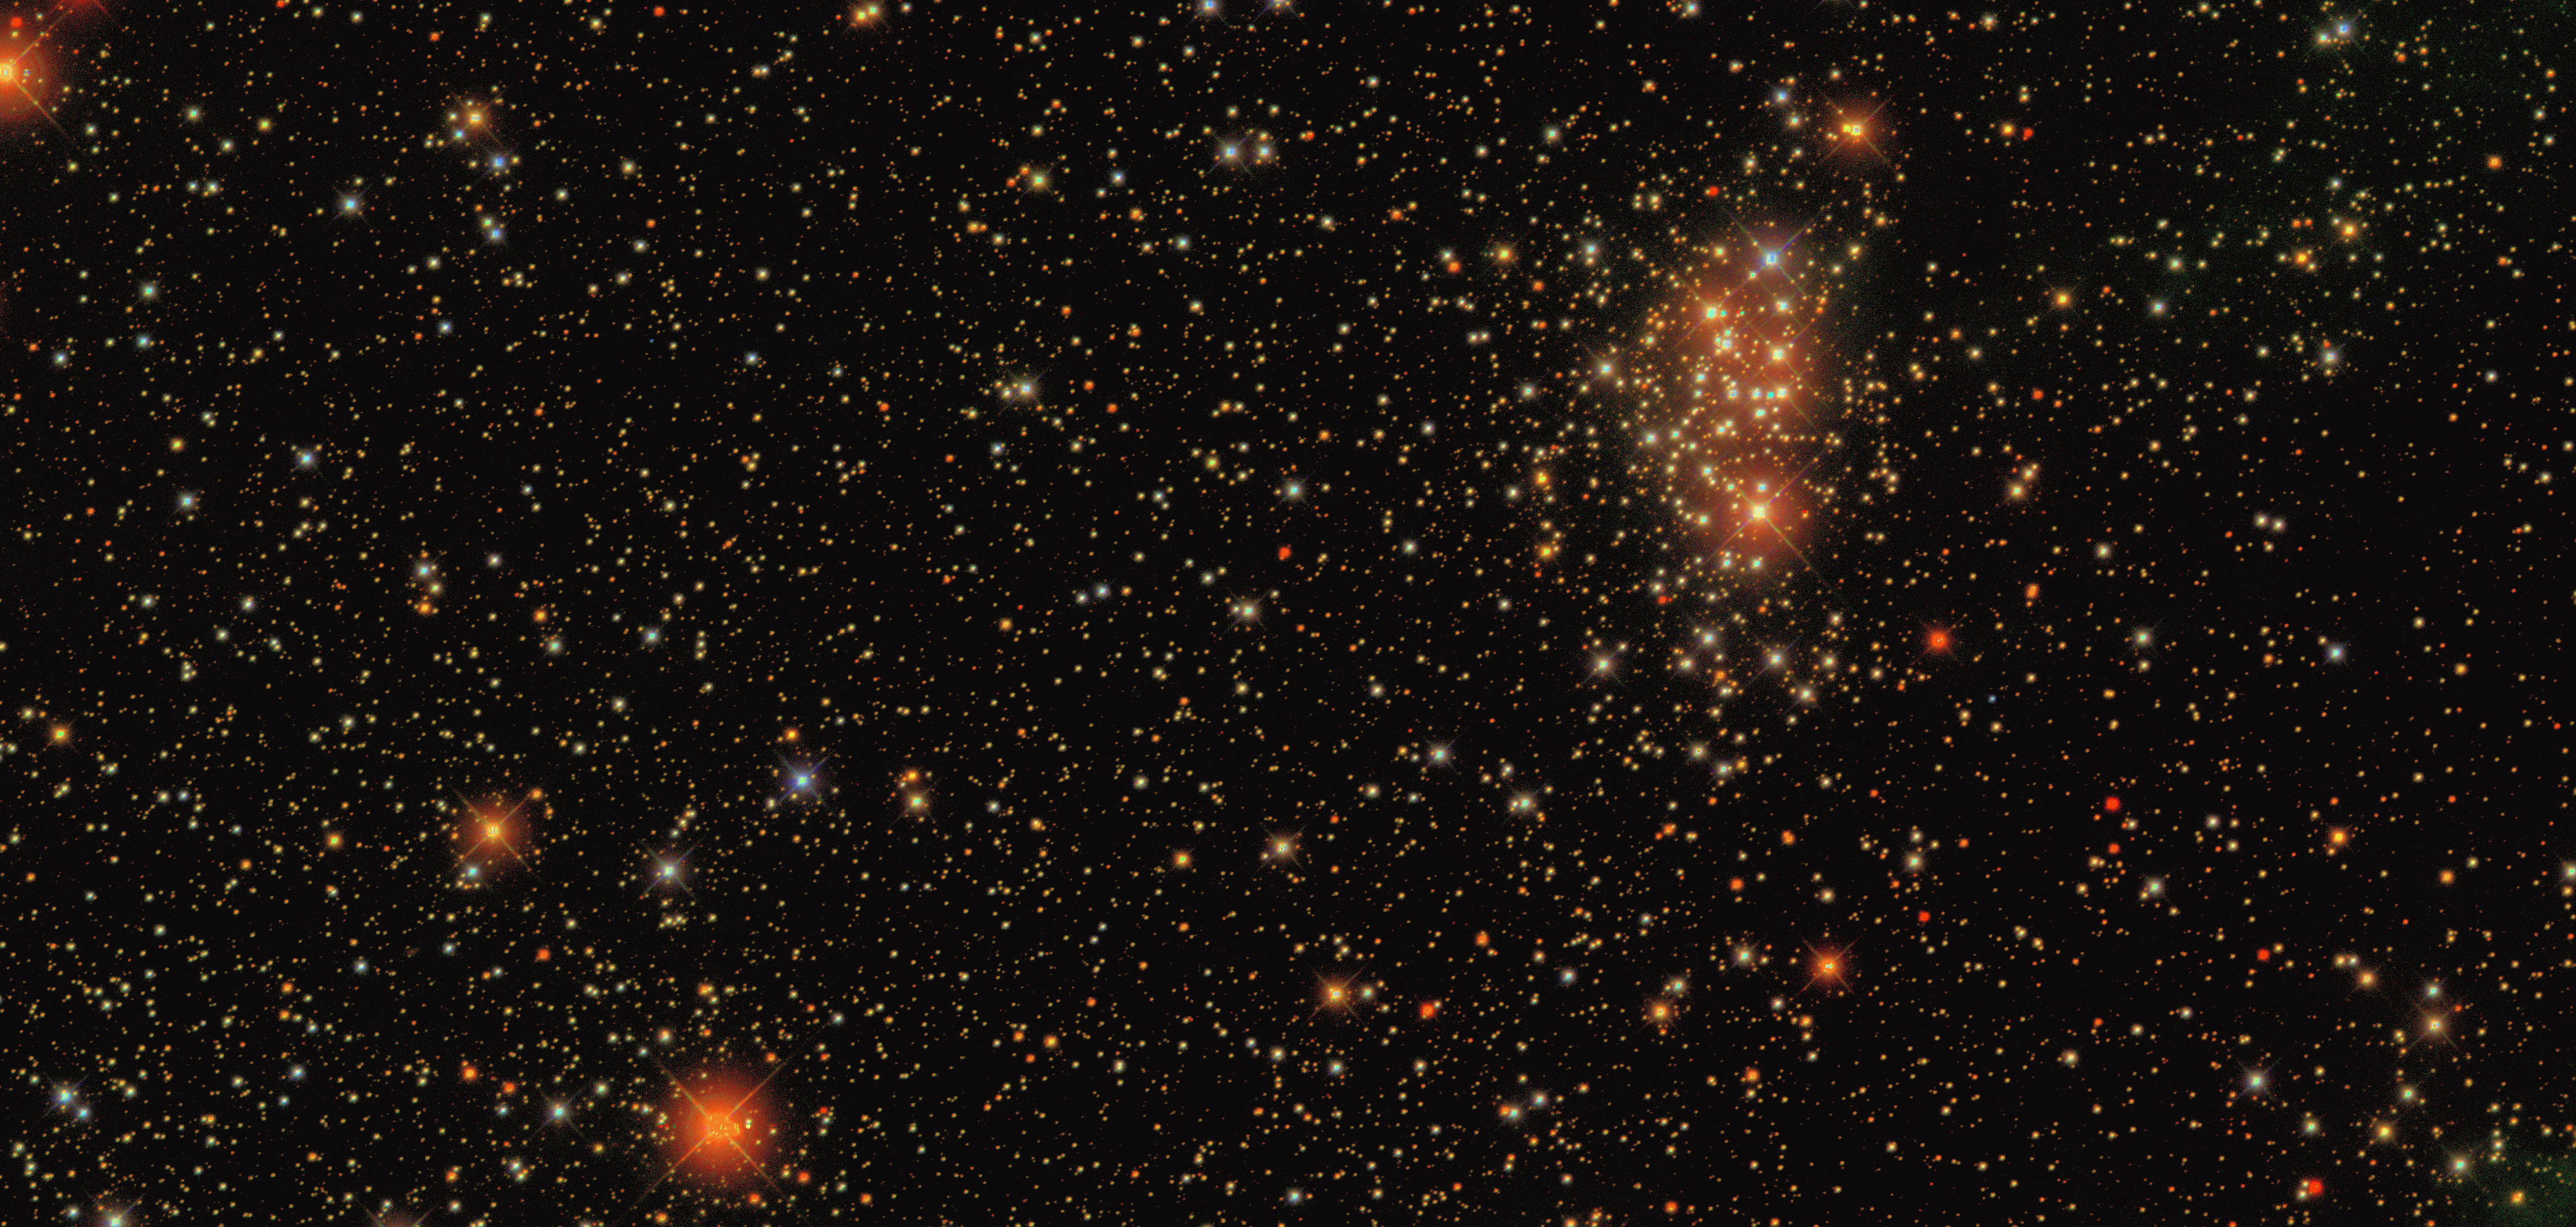
\includegraphics[width=0.6\textwidth]{res/SkyScan.png}
        \caption{Sloan Digital Sky Survey (Robert Lupton)}
    \end{figure}
\end{frame}

\placelogofalse
\frame[plain]{\titlepage}
\placelogotrue

\end{document}
